%% Lab Report for EEET2493_labreport_template.tex
%% V1.0
%% 2019/01/16
%% This is the template for a Lab report following an IEEE paper. Modified by Francisco Tovar after Michael Sheel original document.


%% This is a skeleton file demonstrating the use of IEEEtran.cls
%% (requires IEEEtran.cls version 1.8b or later) with an IEEE
%% journal paper.
%%
%% Support sites:
%% http://www.michaelshell.org/tex/ieeetran/
%% http://www.ctan.org/pkg/ieeetran
%% and
%% http://www.ieee.org/

%%*************************************************************************
%% Legal Notice:
%% This code is offered as-is without any warranty either expressed or
%% implied; without even the implied warranty of MERCHANTABILITY or
%% FITNESS FOR A PARTICULAR PURPOSE! 
%% User assumes all risk.
%% In no event shall the IEEE or any contributor to this code be liable for
%% any damages or losses, including, but not limited to, incidental,
%% consequential, or any other damages, resulting from the use or misuse
%% of any information contained here.
%%
%% All comments are the opinions of their respective authors and are not
%% necessarily endorsed by the IEEE.
%%
%% This work is distributed under the LaTeX Project Public License (LPPL)
%% ( http://www.latex-project.org/ ) version 1.3, and may be freely used,
%% distributed and modified. A copy of the LPPL, version 1.3, is included
%% in the base LaTeX documentation of all distributions of LaTeX released
%% 2003/12/01 or later.
%% Retain all contribution notices and credits.
%% ** Modified files should be clearly indicated as such, including  **
%% ** renaming them and changing author support contact information. **
%%*************************************************************************

\documentclass[journal]{IEEEtran}

\usepackage[italian]{babel}

% *** CITATION PACKAGES ***
\usepackage[style=ieee]{biblatex} 
\bibliography{digital.bib}    %your file created using JabRef
\usepackage{hyperref}
% *** MATH PACKAGES ***
\usepackage{amsmath}
 \usepackage{multirow}

% *** PDF, URL AND HYPERLINK PACKAGES ***
\usepackage{url}
% correct bad hyphenation here
\hyphenation{op-tical net-works semi-conduc-tor}
\usepackage{graphicx}  %needed to include png, eps figures
\usepackage{float}  % used to fix location of images i.e.\begin{figure}[H]

\begin{document}

% paper title
\title{Laboratorio di elettronica digitale\\ 
%\small{1 gennaio 2020}
}

% author names 
\author{\begin{center}Matteo Barbagiovanni\textsuperscript{1},
        Stefano Barbero\textsuperscript{2},
        Federico Malnati\textsuperscript{3},
        Valerio Pagliarino\textsuperscript{4},
        {\small \\
        \textsuperscript{1}
        matteo.barbagiovanni@edu.unito.it -
        \textsuperscript{2}
        stefano.barbero376@edu.unito.it
        \textsuperscript{3}
        federico.malnati@edu.unito.it -
        \textsuperscript{4}
        valerio.pagliarino@edu.unito.it}
        \end{center}}% <-this % stops a space
        
% The report headers
\markboth{Universita' degli Studi di Torino - C.d.L. Triennale in Fisica - 01/01/19 - A.A. 2021-2022    \quad   \quad \quad \quad   \quad \quad \quad  \quad   \quad \quad \quad   \quad \quad LABORATORIO DI ELETTRONICA \quad \quad }%do not delete next lines
{Shell \MakeLowercase{\textit{et al.}}: Bare Demo of IEEEtran.cls for IEEE Journals}

% make the title area
\maketitle

% As a general rule, do not put math, special symbols or citations
% in the abstract or keywords.

\begin{abstract} Testo dell'Abstract
\end{abstract}


\section{Paragrafo}
\IEEEPARstart{T}{esto} di esempio.

\begin{figure*}[t]%[t]
\centering
\begin{center}
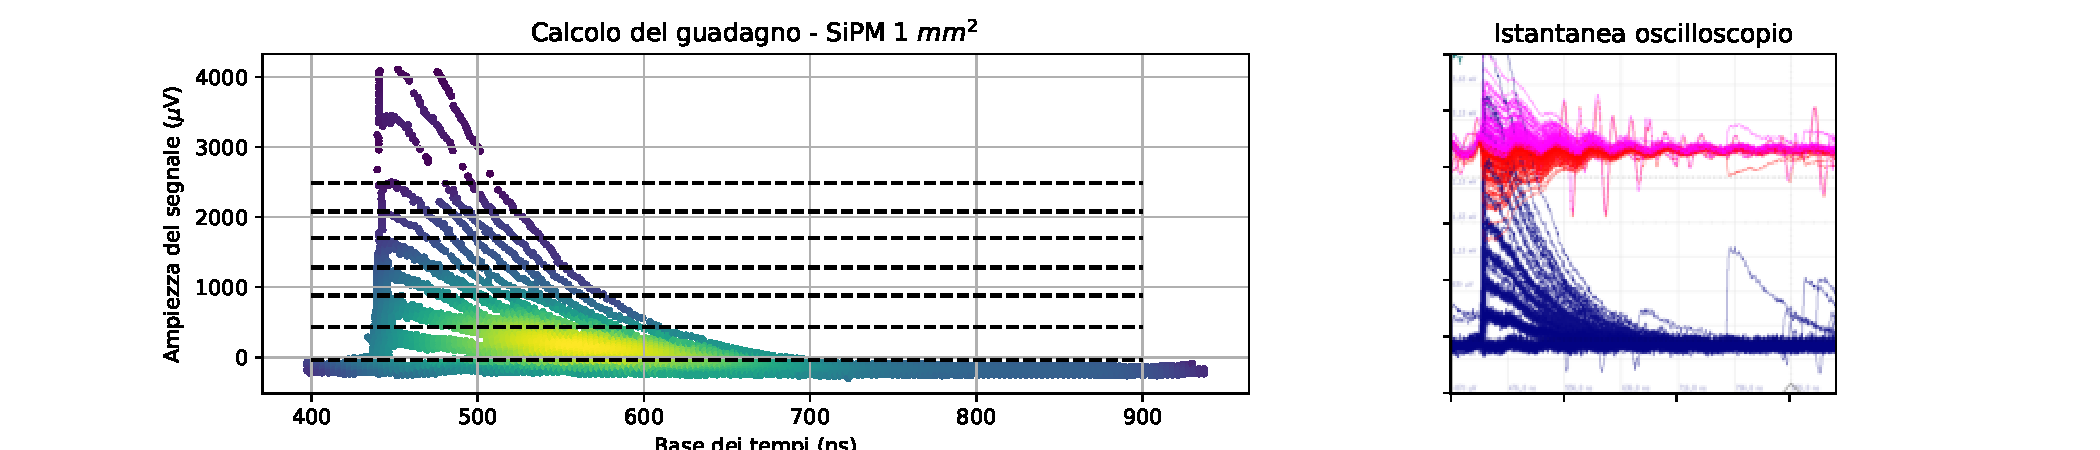
\includegraphics[trim = {100pt 0 0 0}, width=1.15\textwidth]{analysis/output/SiPM_1mm_gain_staircase.pdf}
\end{center}
\caption{A destra l'istantanea catturata dallo schermo dell'oscilloscopio, a sinistra le tracce estratte numericamente sovrapposte con i cursori orizzontali corrispondenti alle tensioni di picco per l'attivazione di N celle. Il gradiente di colore rappresenta invece la densità di tracce. SiPM 1x1 $mm^2$}
\label{fig:staircase_1mm}
\end{figure*}

\end{document}


